% !TEX root = ../main.tex
\chapter{Theory}
The following experiments explore lasers and their applications as well as interference phenomena.

\section{He-Ne Laser}
The common He-Ne-laser consists of a thin (ca. \SI{1}{\milli\meter} in diameter) glass tube filled with a helium-neon gas mixture.
The gas usually is under a pressure of around \SI{100}{\pascal}, the exact mixture of helium and neon depend on the desired wave length of the laser.
At both ends there are resonator mirrors, one of which is partially transparent (to reduce complexity, some lasers use partially transparent mirrors on both ends).
Optional Brewster windows only allow light of one polarization to resonate (see \autoref{sec:brewster}).

To excite the gas atoms, a voltage potential of a few kilovolt applied to the electrodes, which are placed on either end of the tube.
This induces a gas discharge and free electrons can collide with the helium atoms, moving them into an excited state.
The excited helium atoms can stimulate neon atoms, inducing a population inversion among them.
This process is called optical pumping.

Some of the excited neon atoms will spontaneously decay to their ground state, and emit their energy in the form of light.
The light is fed back into the system by the resonator, creating a standing wave.
The standing wave induces stimulated emission, where excited neon atoms create photons of identical phase and wavelength as the standing wave.
This creates highly coherent light with a very narrow spectrum of wavelengths.

\section{Brewster-angle}\label{sec:brewster}

\begin{figure}[tb]
	\centering
	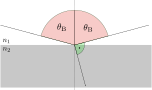
\includegraphics[width=0.6\textwidth]{./img/brewster.pdf}
	\caption[Brewster-angle]{The Brewster-angle}
\end{figure}

Light interacts with dielectric materials (eg. glass) by inducing oscillations in the material's dipoles.
These dipoles can only radiate perpendicular to their axis of vibration.

If the angle between the reflected and the transmitted light is equal to \SI{90}{\degree}, light polarized in the plane of incidence is not reflected, because the dipoles' axis of oscillation is parallel to the direction of transmitted light.

By trivial calculations we can show that
\begin{equation}\label{eq:brewster}
	\tan\theta_\text{B}=\frac{n_2}{n_1},
\end{equation}
where $\theta_\text{B}$ denotes the Brewster-angle and $n_2, n_1$ denote the refraction indices of the material and air respectively (assuming the surface is surrounded by air).

This effect is used inside the He-Ne laser to get a homogenously polarized beam, as s-polarized light is reflected out of the resonance cavity by Brewster windows, whereas light of the other polarization can pass them.

\section{Diffraction phenomena}
The following explanations are of minimal extent, as underlying processes should be familiar.

\subsection{Single slit}\label{subsec:single_slit}

\begin{figure}[tb]
	\begin{subfigure}{.51\textwidth}
		\centering
		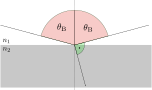
\includegraphics[width=0.6\textwidth]{./img/brewster.pdf}
		\caption[Single slit I]{Path difference deviation}
		\label{fig:path_diff_single}
	\end{subfigure}
	\begin{subfigure}{.51\textwidth}
		\centering
		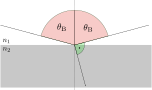
\includegraphics[width=0.6\textwidth]{./img/brewster.pdf}
		\caption[Single slit II]{Angle-distance relation}
		\label{fig:angle_distance_single}
	\end{subfigure}
	\caption[Deviation of single-slit formulae]{Deviation of single-slit formulae}
\end{figure}

Considering \autoref{fig:path_diff_single} we can see that	%I did you ignorant fuck :D (read the '=' sign as 'is equal to' and you'll see)
\begin{equation}\label{eq:path_diff}
	\Delta s=b\sin\alpha
\end{equation}
for the path difference of both beams.

The condition for minima is
\begin{equation}\label{eq:path_diff_min}
	\Delta s = n\cdot\lambda\ ;\qquad n\in\mathbb{N}
\end{equation}
as the transmitted beam is divisible into $2n$ partial beams which cancel out each other in pairs.

The same deliberation can be applied to find the maxima.
It holds
\begin{equation}\label{eq:path_diff_max}
	\Delta s = \left(n+\frac{1}{2}\right)\cdot\lambda\ ;\qquad n\in\mathbb{N}.
\end{equation}
Like this we can divide the beam into $2n+1$ partial beams, the $2n$ beams canceling each other out again, while the last one remains.
This residual beam can be observed as the $n$-th maximum.

Looking at \autoref{fig:angle_distance_single} it holds
\begin{equation}\label{eq:dist_single}
	y_n = d\tan\alpha_n\ ;\qquad n\in\mathbb{N}.
\end{equation}

Assuming the observed angles are small, using equations \ref{eq:path_diff_min}, \ref{eq:path_diff_max} and \ref{eq:dist_single}, we can see that
\begin{equation}\label{eq:single_slit_minima}
	b = \frac{n\lambda d}{y_n} ;\qquad n\in\mathbb{N}.
\end{equation}
for minima and
\begin{equation}\label{eq:single_slit_maxima}
	b = \frac{\left(n+\frac{1}{2}\right)\lambda d}{y_n} ;\qquad n\in\mathbb{N}.
\end{equation}
for maxima of the diffraction pattern.

\subsection{Bridge}\label{subsec:bridge}
To deduce the diffraction pattern of a bridge, we make use of Babinet's theorem which states that two complementary objects have the same diffraction pattern.
This can be understood considering following thoughts:
Assuming $O$ is the original diffracting object and $\bar{O}$ is its complement viz. that it is opaque where $O$ is transparent and vice versa.
The sum of the amplitudes by the diffractions caused by $O$ and $\bar{O}$ must equal the amplitude of an unobstructed beam.
This means that in places where the light would not have reached without diffraction, the phases of patterns caused by $O$ and $\bar{O}$ must be opposite in phase, effectively causing the amplitude to be negative.
However, for perception of the diffraction patterns not amplitude matters but intensity, which is proportional to the square of the amplitude.

We notice that a bridge of thickness $b$ is the complement of a single-slit of same gap-width, so the diffraction patterns should be the same and we can use the same equations as deviated in \autoref{subsec:single_slit}.

\subsection{Circular disk and opening}
Due to Babinet's principle, the observed diffraction patterns of a disk and a circular opening of same width should be the same.
We expect rotationally symmetrical patterns.

\subsection{Hair}
A hair poses the same object as elaborated in \autoref{subsec:bridge} so according formulae can be applied to calculate its width.

\subsection{Double-slits}
The interference pattern of a double-slit can be explained via the Huygens-Fresnel principle.
It states that each point on a wavefront generates a secondary wavelet and that the disturbance at any subsequent point can be found by summing the contributions of the individual wavelets at that point.
Assuming both slits are small compared to the wavelength of the laser, they diffract light into new cylindrical wavelets which superimpose at their amplitude and hence their intensity.

As in \autoref{eq:path_diff}, it holds
\begin{equation*}
	\Delta s=g\sin\alpha,
\end{equation*}
$g$ denoting the distance between the two parallel slits.
This time, however, there only are two beams as our earlier assumption guarantees, so the conditions for maxima and minima are altered.

The condition for maxima becomes
\begin{equation}\label{eq:double_path_max}
	\Delta s = n\cdot\lambda\ ;\qquad n\in\mathbb{N},
\end{equation}
whereas
\begin{equation}\label{eq:double_path_min}
	\Delta s = \left(n+\frac{1}{2}\right)\cdot\lambda\ ;\qquad n\in\mathbb{N}.
\end{equation}
can be found for minima.
Note that these are the same conditions as in \autoref{subsec:single_slit}, yet flipped. \todo{swapped? however? only? You decide.}

Using \autoref{eq:dist_single}, this leads to

\begin{alignat}{3}
 	g &= \frac{n\lambda d}{y_{\text{max,}n}} &\quad n\in\mathbb{N},\label{eq:double_max} \\
	g &= \frac{\left(n+\frac{1}{2}\right)\lambda d}{y_{\text{min,}n}} &\quad n\in\mathbb{N}, \label{eq:double_min}
\end{alignat}
where $y_{\text{max,}n}$ and $y_{\text{min,}n}$ denote the position of the $n$-th maximum and minimum respectively.

\subsection{Lattices}\label{subsec:lattices}
Noting that lattices are just $n$ subsequent slits placed in intervals of $\frac{1}{g}$, we can deduce that
\begin{alignat}{3}
 	\frac{1}{g} &= \frac{n\lambda d}{y_{\text{max,}n}} &\quad n\in\mathbb{N},\label{eq:lattice_max} \\
	\frac{1}{g} &= \frac{\left(n+\frac{1}{2}\right)\lambda d}{y_{\text{min,}n}} &\quad n\in\mathbb{N}, \label{eq:lattice_min}
\end{alignat}
holds for the maxima and minima as in equations \ref{eq:double_max} and \ref{eq:double_min}.
For all kinds of slits used in this experiment, however, the exact relation viz. $n$ or $\left(n+\frac{1}{2}\right)$ does not matter in a plot order vs. distance between features, since only the slope is of interest to determine distance between slits or gap width respectively.
Hence, measuring distances between maxima or minima does not matter, since it only causes an offset but does not change the slope.

\section{Holograms}\label{sec:holograms}
Ordinary photographs are created by projecting an illuminated object with a lens system onto a plane, reducing the dimension of the object by one (3D$\rightarrow$2D).
All information about phase of the incident light is lost in this process.
However, \texttt{Denis Gabor}$\dagger$ had the idea of superimposing two waves, the so called \textbf{reference wave} and the wave scattered by the illuminated body, at a photo plate, retaining all information about phase and amplitude of the scattered object wave and hence the three-dimensional geometry of the body.
This method uses a coherent light source i.e. a laser.
First, the beam is widened by a lens and then split by a beam splitter.
The first partial beam is pointed directly onto the photo plate, while the second one illuminates the body.
The beam scattered by this object in the direction of the photo plate has a phase shift subject to the distance of the individual object points from the photo plate.
This dependence contains the desired information about the geometry of the object (distance of the individual object points).
The interference pattern created on the plate, however, has no resemblance with the actual body at all.
To make it visible again, the photo plate is illuminated by a light source of the same wavelength and now can be viewed from different angles, revealing different sides of the imaged object.

\section{Measurements, Calculation of Feature Size and Error}\label{sec:meas}
\begin{figure}[tb]
	\centering
	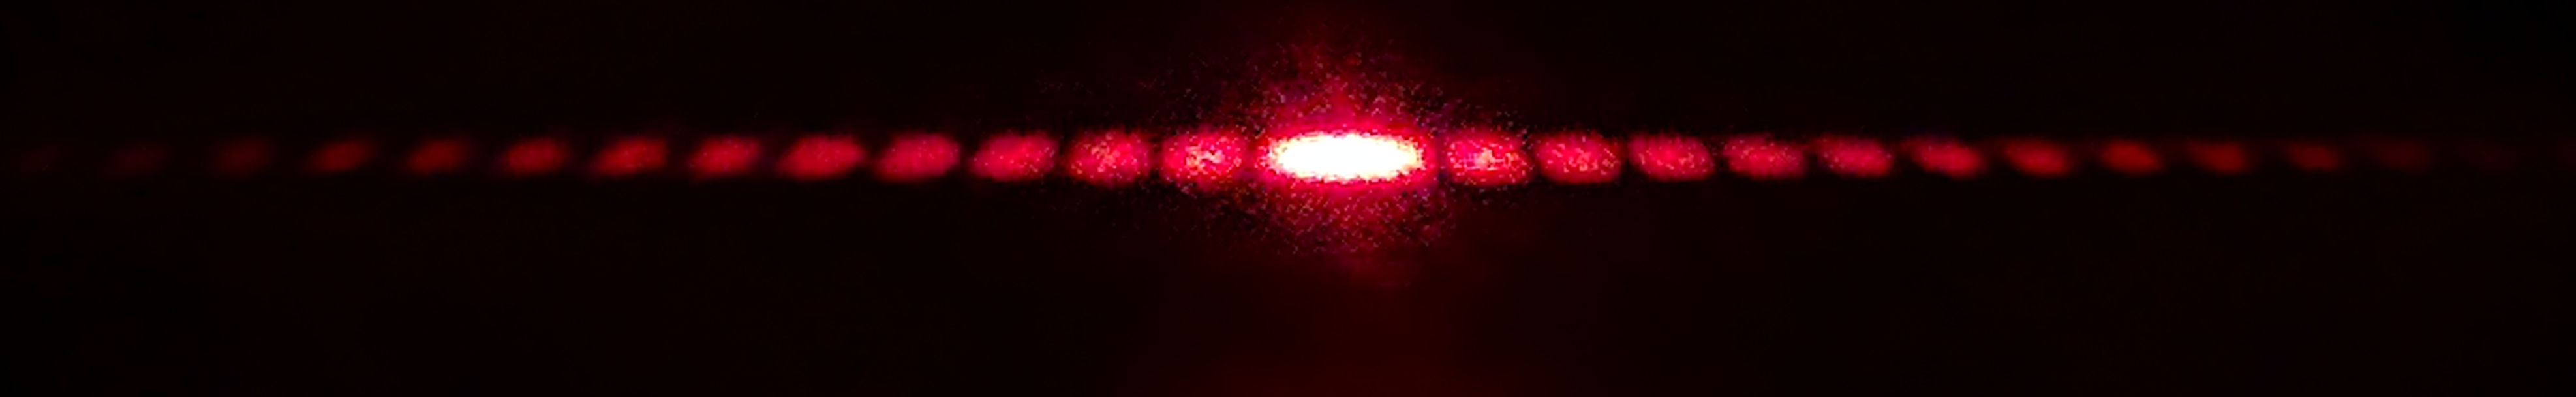
\includegraphics[width=0.6\textwidth]{./img/diffraction.pdf}
	\caption{Typical Diffraction Pattern}
	\label{fig:diffraction}
\end{figure}
Despite the very different geometries of the experiments, the feature size $W$ (the width of a single slit or the spacing of a double slit or optical grating) can be calculated using the same method:

The distances $d_{1 \dots m}$ between the two peaks or troughs of the first m diffraction orders are measured by hand and converted to the deflection angles using $\alpha_n = \frac{d_n}{2 D_\text{screen}}$, where $D_\text{screen}$ is the distance between object and screen.\\
A linear fit $\alpha_n = S \cdot n + d_0$ is applied to the angles.
The feature size $W$ is calculated by $W = \frac{\lambda}{S}$.

The error in $S$ is calculated using the fitting tool \textit{kafe}\footnote{\url{https://github.com/dsavoiu/kafe}}, assuming uncorrelated statistical errors of \SI{1}{\mm} for the distances $d_n$ and \SI{10}{\mm} for $D_\text{screen}$.


Another error source is the wavelength $\lambda$ of the He-Ne laser.
The wavelength of a He-Ne laser typically lies within \SI{2}{\ppm} of the standard $\lambda_0 = \SI{632.816}{\nm}$ (in air)\footnote{\url{http://www.k3pgp.org/Notebook/Lasersam/laserhen.htm\#hentoo0}}.
As $\lambda$ is proportional to $W$, this error translates directly to the error in $W$.
This statistical error is much smaller than the error introduced by $S$, so it can safely be disregarded.

Since there is only one error source for $W$, the error in $W$ is calculated by $\sigma_W = W \cdot \frac{\sigma_S}{S}$.

Some measurements were repeated with different distances $D_{screen}$, the mean is calculated by weighting the individual values with the inverse square of their respective errors.
The error in the mean value is $\sigma_\text{mean} = \left(\sum_{n = 1}^m (\sigma_n^{-2})\right)^{-\frac{1}{2}}$
